% !TeX spellcheck = en_US
\documentclass{report}
\usepackage{paccosp}
	\makeindex
\begin{document}
	\title{Stochastic Processes notes}
	\author{Kotatsu}
	\date{\small vaffanculo}
	\maketitle
	\pagenumbering{Roman}
	\begin{preface}
Let's have a fucking party!
		
		\vskip1.2cm
		
		\hfill Kotatsu
	\end{preface}
	\clearpage
	\tableofcontents
	\pagenumbering{arabic}
\chapter{Brownian Motion}	
	\section{Continuity of stochastic processes}
	The sample path in a discrete scenario is given by
	\begin{equation*}
		\pr(X(t)<x|\F_{s})=\pr(X(t)<x|X_{s}).
	\end{equation*}
	This gives us a sample path like this:
	\begin{figure}[H]
		\centering
		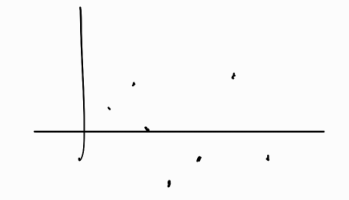
\includegraphics[width=0.7\linewidth]{img/screenshot003}
		\caption{Fucking hell.}
		\label{fig:screenshot003}
	\end{figure}
	We want to think, though, about a continuous space and time process: 
	\begin{figure}[H]
		\centering
		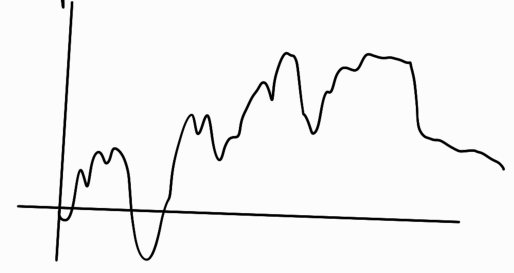
\includegraphics[width=0.7\linewidth]{img/screenshot004}
		\caption{Leaning like my academic career.}
		\label{fig:screenshot004}
	\end{figure}
	How can we define the continuity of the sample paths? and how can we check this property? There are some possible definitions of continuity. To control for their robustness we check whether according to each of these definitions the Poisson process, a discrete process, is correctly classified as non continuous.
	\begin{definition}
		A stochastic process $\{M(t)\}$ is said to be a \emph{counting process} if:
		\begin{enumerate}[i.]
			\item $M(t)>0$;
			\item $M(t)$ is an integer;
			\item $M(t)$ is increasing, meaning that $s\leq t\implies M(s)\leq M(t)$.
		\end{enumerate}
	\end{definition}
	In general, these processes count how many times an event happens.
	\begin{definition}
		A Poisson process is a counting process such that:
		\begin{enumerate}
			\item $N(0)=0$;
			\item for $t_1<t_2<t_3<t_4$ we have
			\begin{equation*}
				N(t_2)-N(t_1)\independent N(t_4)-N(t_3)
			\end{equation*}
			meaning that the increments are independent;
			\item for $\every h>0$ and $t>\tau$ it holds:
			\begin{equation*}
				N(t)-N(\tau)\sim N(t+h)-N(\tau+h)
			\end{equation*}
			meaning that the increments are stationary (the origin start doesn't matter);
			\item we have $$\pr(N(t)=k)=\frac{(\lambda t)^{k}}{k!}e^{-\lambda t}\qquad\text{for } k=0,1,\ldots$$
		\end{enumerate}
	\end{definition}
	\begin{figure}[h]
		\centering
		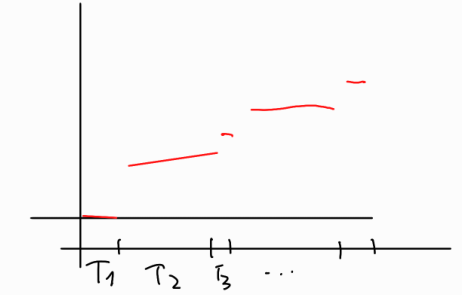
\includegraphics[width=0.7\linewidth]{img/screenshot002}
		\caption{I am very good at drawing straight lines.}
		\label{fig:screenshot002}
	\end{figure}
	
	The inter-arrival times are i.i.d. \rv s distributed as
	\begin{equation*}
		T_i\distexp{\lambda}.
	\end{equation*}
	The continuity of sample paths can be characterized in four different ways:
	\begin{enumerate}
		\item \emph{Continuity in mean squares}: we have this if for $\every t\geq0$ we have
		\begin{equation*}
			\lim_{s\to t}\ev\left[|X(t)-X(s)|^{2}\right]=0.
		\end{equation*}
		So according to this definition, the mean square of the distance goes to 0 if we go near $s$.
		\item \emph{Continuity in probability}: we have this if for $\every t\geq0$ and $\every\varepsilon>0$ we have
		\begin{equation*}
			\lim_{s\to t}\pr(|X(t)-X(s)|>\varepsilon)=0.
		\end{equation*}
		This should be enough for all finite distributions, right?\footnote{First, but not last, question without an answer.}
		\begin{theorem}
			Let $\{X(t)\}$ be a stochastic process such that $\ev[X^{2}(t)]<\infty$ for all $t$. Then it is continuous in mean squares\ifonly{}:
			\begin{enumerate}
				\item $m(t)=\ev[X(t)]$ is continuous;
				\item the covariance function
				\begin{equation*}
					\Gamma(s,t)=\ev[(X(t)-m(t))(X(s)-m(s))]
				\end{equation*}
				is continuous on its diagonal set.
			\end{enumerate}
			\begin{fancyproof}
				Consider the expectation
				\begin{equation*}
					\ev\left[|X(t)-X(s)|^{2}\right]=\ev\left[|X^{2}(s)+X^{2}(t)-2X(t)X(s)|\right]\tag{\faAdjust}\label{boh}
				\end{equation*}
				but
				\begin{equation*}
					\ev\left[X^{2}(s)\right]=\ubracketthin{\ev\left[(X(s)-m(s))^{2}\right]}_{\Gamma(s,s)}+2m(s)\ev\left[X(s)\right]-m^{2}(s)
				\end{equation*}
				and
				\begin{equation*}
					\ev\left[X^{2}(t)\right]=\Gamma(t,t)+2m(t)\ev[X(t)]-m^{2}(t)
				\end{equation*}
				and, moreover,
				\begin{equation*}
					\ev[X(s)X(t)]=\Gamma(s,t)-\cancel{m(t)m(s)}+m(t)\ev[X(s)]+\cancel{m(s)\ev[X(t)]}.
				\end{equation*}
				So \ref{boh} becomes
				\begin{align*}
					\text{\faAdjust}&=\Gamma(s,s)+2m^{2}(s)-m^{2}(s)+\Gamma(t,t)+2m^{2}(t)-m^{2}(t)-2\ev\left[X(s)X(t)\right]\\
					&=\Gamma(s,s)+\Gamma(t,t)-2\Gamma(s,t)+m^{2}(t)+m^{2}(s)-2m(t)m(s)\\
					&=\Gamma(s,s)+\Gamma(t,t)-2\Gamma(s,t)+\left[m(t)-m(s)\right]^{2}.
				\end{align*}
				Hence, if $m(t)$ is continuous and $\Gamma(s,t)$ is continuous for $s=t$ then the process is continuous because we have:
				\begin{itemize}
					\item $[m(t)-m(s)]^{2}\to0$ since it is a continuous function;
					\item $\Gamma(s,s)+\Gamma(t,t)-2\Gamma(s,t)$ that becomes $\Gamma(t,t)+\Gamma(t,t)-2\Gamma(t,t)=0$.
				\end{itemize}
				I'd like to add that dear prof. Sacerdote didn't explain this last little point. Thank you! So now whe have
				\begin{equation*}
					\ev\left[|X(s)-X(t)|^{2}\right]\to0.
				\end{equation*}
				If this holds for $m(t)$ and $\Gamma(t,t)$ then it is continuous in mean squares.
			\end{fancyproof}
		\end{theorem}
		\begin{remark}
			A process continuous in mean \faSquare[regular] (get it?) is continuous in probability (use Chebyshev\footnote{Like use him? As a person? He is dead.}).
		\end{remark}
		Is the Poisson process continuous in mean \faSquare[regular] (and also in probability)? We know that
		\begin{equation*}
			m(t)=\lambda t
		\end{equation*}
		and 
		\begin{align*}
			\Gamma(s,t)&=\ev[(N(t)-m(t))(N(s)-m(s))]\\
			&=\ev[N(t)N(s)]-2m(t)m(s)-m(t)m(s)\\
			&\underset{t>s}{=}\ev[(N(t)-2N(s)+N(s))N(s)]-m(t)m(s)\\
			&=\ev[(N(t)-N(s))N(s)]+\ev\left[N^{2}(s)\right]-m(t)m(s)\\
			&=\ubracketthin{\ev[N(t)-N(s)]}_{
			\lambda(t-s)}\ubracketthin{\ev(N(s))}_{\lambda s}+\ev\left[N^{2}(s)\right]-\ubracketthin{m(t)}_{\lambda t}\ubracketthin{m(s)}_{\lambda s}\\
			&=\lambda^{2}(\cancel{t}-s)s-\cancel{\lambda^{2}ts}+\ev\left[N^{2}(s)\right]\\
			&=-\lambda^{2}s^{2}+\ubracketthin{\var N(s)}_{\lambda s}+\ubracketthin{\left[\ev\left[N(s)\right]\right]^{2}}_{\lambda^{2}s^{2}}\\
			&=\lambda s\qquad\text{if }s<t.
		\end{align*}
	\begin{figure}[h]
		\centering
		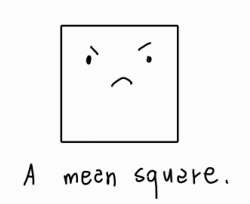
\includegraphics[width=0.3\linewidth]{img/screenshot001}
		\caption{Sei un fallito.}
		\label{fig:screenshot001}
	\end{figure}
	So $\Gamma(s,t)=\lambda\min(s,t)$ is continuous on diagonal and $m(t)=\lambda t$ is also continuous... but this would mean that Poisson processes are continuous! Which they shouldn't be! Do I care? No!
	\item \emph{Almost sure continuity}: we can ask, as a requirement, that
	\begin{equation*}
		\pr\left(\lim_{s\to t}N(s)=N(t)\right)=1.
	\end{equation*}
	Does this finally solve the problem with the Poisson processes? No, because it verifies the almost sure continuity (since it is discontinuous only in a countable number of instances).\\
	It is not enought ot think point by point: we must think \textit{uniformly}.
	\begin{definition}
		A stochastic process $\{X(t)\}$ has almost sure continuous sample paths if, with probability 1, $X(t)$ is a continuous function, that is:
		\begin{equation*}
			\pr(X(t)\text{ has continuous samples})=1.
		\end{equation*}
	\end{definition}
	Of course, the case in which you have exceptional points is not a problem since they have measure 0.
	\begin{figure}[h]
		\centering
		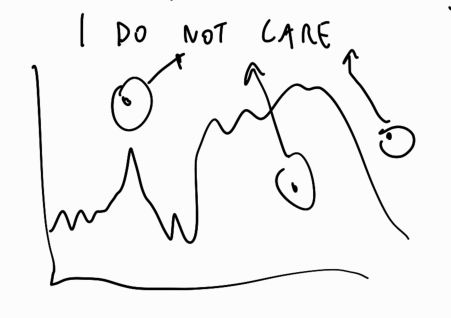
\includegraphics[width=0.4\linewidth]{img/screenshot005}
		\caption{Me neither.}
		\label{fig:screenshot005}
	\end{figure}
	\begin{remark}
		The set
		\begin{equation*}
			\{\omega\in\Omega:t\to B_{t}(\omega)\text{ is continuous}\}
		\end{equation*}
		is not necessarily in the \sa{} generated by the vectors
		\begin{equation*}
			\left(B_{t_{1}}, B_{t_{2}},\ldots,B_{t_{n}}\right)\qquad n\in\N.
		\end{equation*}
	\end{remark}
\end{enumerate}
\section{Definition of Brownian motion}
Imagine a spherical particle with a diameter of $10^{-6}$ m surrounded by $10^{-23}$ (the Avogadro number) molecules with a diameter of $10^{-10}$ m of diameter.
\begin{figure}[h]
	\centering
	\begin{tikzpicture}
		\shade[ball color = gray!40, opacity = 0.4] (0,0) circle (1.2cm);
		\draw (0,0) circle (1.2cm);
		\draw (-1.2,0) arc (180:360:1.2 and 0.6);
		\draw[dashed] (1.2,0) arc (0:180:1.2 and 0.6);
		\fill[fill=black] (0,0) circle (1pt);
		\draw[dashed] (0,0 ) -- node[above]{\tiny$10^{-6}\;m$} (1.2,0);
		\foreach \a in {1,2,...,17}{
			\draw (\a*360/17: 2cm) circle (0.2cm);
			\shade[ball color=Green3,opacity=0.6] (\a*360/17: 2cm) circle (0.2cm);
		}
	\end{tikzpicture}
	\caption{My balls.}
	\label{fig:screenshot006}
\end{figure}
How can we model the behavior of this ball in a mathematical way\footnote{At this point of the lesson Prof. Sacerdote started ranting about Machine Learning (seriously?) being a black box for like 10 minutes.}?\\
In 1828 Robert Brown (fig. \ref{fig:autecre}) observed the chaotic movement of pollen in the water through a microscope and noted:
\begin{itemize}
	\item the motion was composed by translations and rotations;
	\item particles seemed to move independently one from the other;
	\item smallest particles moved more actively;
	\item less viscous fluids determined more activity movement;
	\item the motion never ceased;
	\item the motion was not determined by liquid flows or evaporation;
	\item particles were not animated.
\end{itemize}
In 1905 Einstein gave the correct explanation formulating a model that also proved valid for forecasting: the idea was that the atoms surrounding the particles (the atoms of the fluid) performed a temperature-dependent movement that collided with the particles, changing their direction.\\
\begin{figure}[h]
	\centering
	
\includegraphics[width=0.5\linewidth]{img/screenshot006}
	\caption{Autechre are a IDM duo from Rochdale, England, composed by Robert Brown and Sean Booth.}
	\label{fig:autecre}
\end{figure}
In 1906 the Polish mathematician Smoluchowski independently obtained results similar to Einstein's. Unrelated, but in 1909 Jean Perrin determined the size of atoms.\\
The Einstein approach considers the motion of a particle over a small interval $T$ observed in a time large enough to see at least 2 intervals $t$ independent. Consider, for the sake of simplicity, the one-dimensional case. During $t$ the particle moves of a distance $\Delta$, that is a \rv{} with density $\varphi(\Delta)$ that must be symmetric so $\varphi(\Delta)=\varphi(-\Delta)$. For example, we can imagine $\varphi(\Delta)\sim\mathsf{N}$ with mean 0 (since in this model we do not expect a drift) and small variance. Then we can consider
\begin{equation*}
	\gamma=f(x,t)\qquad\text{as the number of particles per unit of volume.}
\end{equation*}
Einstein proved that $f$ verifies
\begin{equation*}
	\frac{\partial f}{\partial t}=D\frac{\partial^{2}f}{\partial x^{2}}.
\end{equation*}
This was the equation of heat diffusion that was already well known at the time. And so was its solution, which is
\begin{equation*}
	f(x,t)=\frac{1}{\sqrt{4\pi Dt}}e^{-\frac{x^{2}}{4Dt}}.
\end{equation*}
In this case $D$ had a physical meaning: Einstein proved\par
\noindent
\begin{minipage}{0.5\textwidth}
	\begin{equation*}
		D=\frac{1}{\sqrt{6\pi r\eta}}\frac{RT}{N}
	\end{equation*}
\end{minipage}\begin{minipage}{0.5\textwidth}
\begin{itemize}
	\item $\eta$: dynamic viscosity
	\item $r$: dimension of particles
	\item $R$: gas constant (8.3 $\frac{\mathrm{J}}{\mathrm{mol~K}}$)
	\item $T$: absolute temperature
	\item $N$: Avogadro's number
\end{itemize}
\end{minipage}
\clearpage
\listoffigures  
\end{document} 


%THIS IS THE DARK AGE OF LOVE   